\begin{enumerate}
	\item Exercício
	
	Encontre o volume do sólido limitado pelas funções abaixo.
	
	\begin{equation*}
		z  = x^2 + y^2	
	\end{equation*}
	\begin{equation*}
		z = 9
	\end{equation*}
	
	\begin{figure}[htb]
		\caption{Coordenadas cilíndricas - Aula 01 - Exercício I}
		\label{v25_a01_e01}
		\centering
		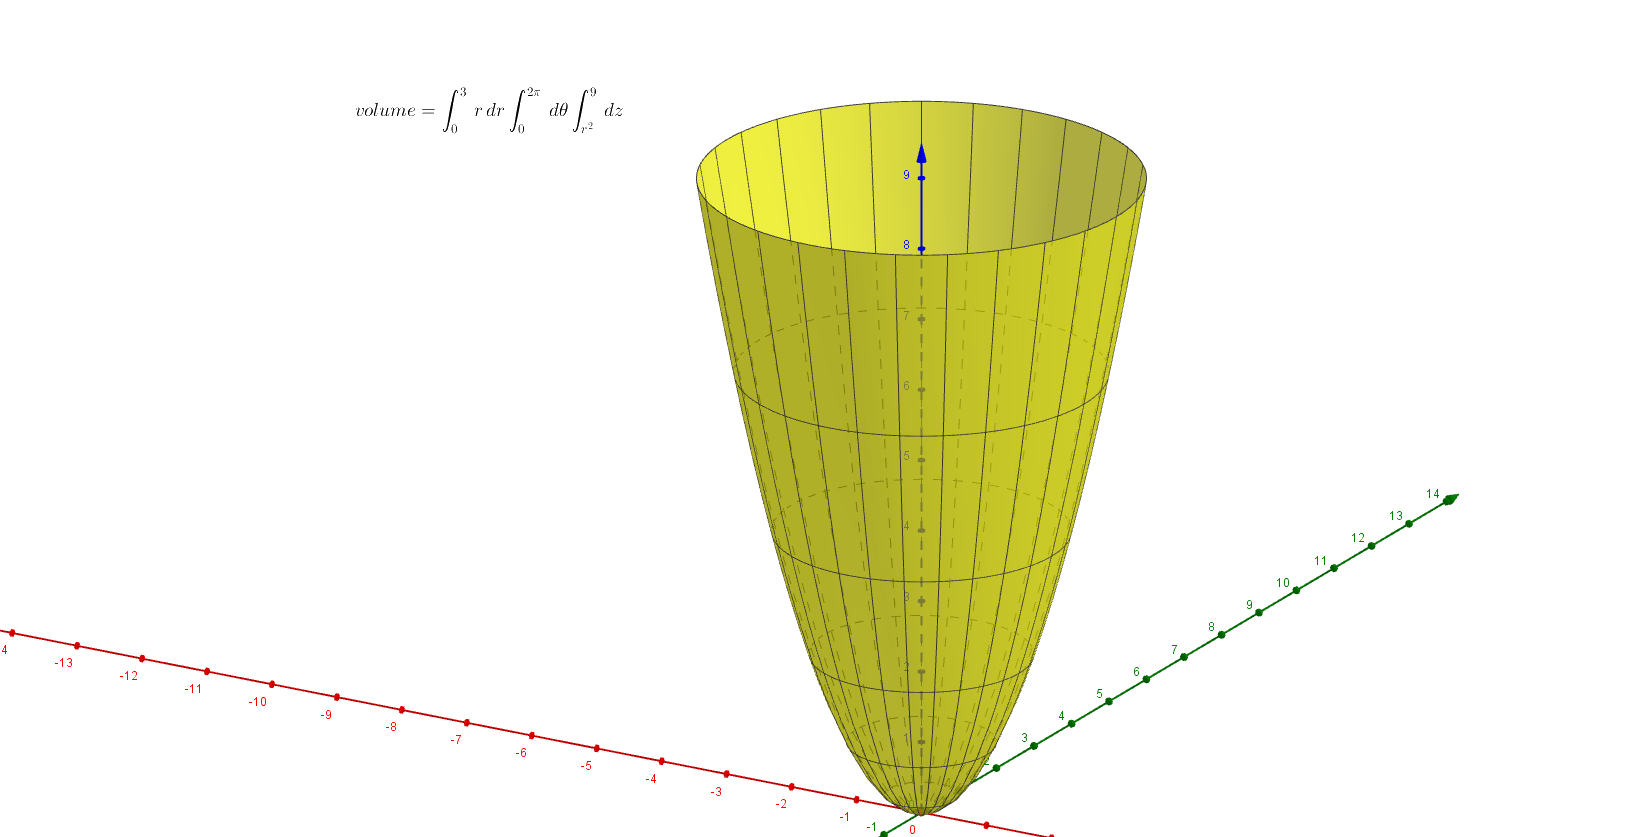
\includegraphics[width=0.5\textwidth]{v25_a01_e01.png}		
	\end{figure}
		
	\begin{equation*}
		z  = x^2 + y^2 = r^2	
	\end{equation*}
	\begin{gather*}
		x^2 + y^2 = r^2 = 3^2 = 9
	\end{gather*}
	\begin{equation*}
		0 \leq r \leq 3,\, 0 \leq \theta \leq 2\pi,\, r^2 \leq z \leq 9
	\end{equation*}
	\begin{gather*}
		\int_0^3 \int_0^{2\pi} \int_{r^2}^9 r\, dz d\theta dr = \int_0^3 r\, dr \int_0^{2\pi} d\theta \int_{r^2}^9 dz = \int_0^3 r\, dr \int_0^{2\pi} d\theta \left[z\right]_{r^2}^9 =\\ \int_0^3 r\left(9 - r^2\right)\, dr \int_0^{2\pi} d\theta = \int_0^3 \left(9r - r^3\right)\, dr \int_0^{2\pi} d\theta = \left[\dfrac{9r^2}{2} - \dfrac{r^4}{4}\right]_0^3 \left[\theta\right]_0^{2\pi} =\\ \left[\dfrac{18r^2 - r^4}{4}\right]_0^3 2\pi = \dfrac{\pi}{2}\left[r^2\left(18 - r^2\right)\right]_0^3 = \dfrac{\pi}{2}9\left(18 - 9\right) = \dfrac{81\pi}{2}
	\end{gather*}		
\end{enumerate}